\section{Higgs-Mechanismus (10P)}
\begin{enumerate}
\item 
    Im Juli 2012 wurden die Ergebnisse der Suche nach dem Higgs-Boson von der ATLAS und CMS Kollaboration veröffentlicht. Beide Experimente fanden das Teilchen bei einer Masse von ungefähr $\SI{125}{\giga\electronvolt\per c\squared}$. Aktuelle Daten, die bei höheren Schwerpunktsenergien aufgenommen wurden, bestätigen dieses Ergebnis.
    
    Was ist das Higgs-Boson und warum ist es ein fundamentaler Teil des Standardmodells? (1P)
    
  \solution{
  In July 2012 the ATLAS and CMS collaborations announced their results for the Higgs search at CERN. Both discovered the Higgs boson at a mass of around \SI{125}{\giga\electronvolt\per c\squared}. The current data at higher center of mass energies confirm this result. 
  
  What is the Higgs Boson and why is it fondamental in the Standard Model?

  The higgs bosons is a fundamental particle of the standard model responsible to the mechanism by which all the fermions and the Z, $W^\pm$ bosons acquire mass.
           }
\item
    Definieren Sie die beiden komplexen Skalarfelder, die das Higgs beschreiben und erklären Sie den Higgs-Mechanismus grob. (2P)

  \solution{
    Define the two complex scalar Higgs fields and give a roughly explanation of the idea behind the Higgs mechanism.

    The two complex scalar fields, placed in a weak isospin douplet are $\phi^+$ and $\phi^0$. The Higgs mechanismn is comes from the Spontaneous symm breaking of a complex scalar field with a potential $V(\phi)= \mu^2\phi^2+\lambda\phi^4$ embedded with a local gauge symmetry of the group $U(1)_Y \times SU(2)_L$
           }
%\item
%    Betrachten Sie die Terme des Lagrangian, der die Wechselwirkung zwischen den physikalischen $W^+$ und $W^-$ Feldern und dem Higgs-Boson beschreibt. 
%    \begin{equation}
%    \mathcal{L}=\frac{1}{4}g^2_Wv^2W_\mu^-W^{+\mu}+\frac{1}{2}g^2_WvW_\mu^-W^{+\mu}h+\frac{1}{4}g^2_WW_\mu^-W^{+\mu}hh
%    \end{equation}
%    Hierbei ist $v$ der Vakuum-Erwartungswert, an dem das Higgs-Potential sein Minimum hat,
%    $g_W$ ist die Yukawa-Kopplung und $h$ das physikalische Higgs-Boson.
%    Welcher dieser Terme ist für die Masse der $W^+$ und $W^-$ Bosonen verantwortlich?
%    Zeichnen Sie die Feynman-Diagramme der anderen beiden Terme.

%  \solution{
%    Consider the terms of the Lagrangian which describe the interaction of the physical $W^+$ and $W^-$ fields with the Higgs boson
%    \begin{equation}
%    \mathcal{L}=\frac{1}{4}g^2_Wv^2W_\mu^-W^{+\mu}+\frac{1}{2}g^2_WvW_\mu^-W^{+\mu}h+\frac{1}{4}g^2_WW_\mu^-W^{+\mu}hh,
%    \end{equation}
%    where $v$ is the non-zero vacuum expectation value at which the Higgs potential is at minimum, $g_W$ is the Yukawa coupling and $h$ is the %"physical" Higgs Boson. Which one of these terms is responsible to the non-zero mass of the $W^+$ and $W^-$ bosons? Draw the Feynman diagrams of the other two terms.

%    The term resposible for the non-zero mass of the W is the first one, proportional to the $v^2$ the other two are triple and quadratic %couplings between one or two Higgs boson and the gauge bosons. 
%           }
\item 
    Im Prinzip kann das Higgs-Boson in alle Teilchen des Standardmodells zerfallen. 
    Allerdings sind aufgrund ihrer großen Verzweigungsverhältnisse nur sechs Zerfallskanäle
    relevant. Welche Zerfallskanäle sind dies und welcher davon tritt am häufigsten auf? Begründen Sie kurz, warum dieser Kanal am häufigsten auftritt. Zeichnen Sie die Feynman-Diagramme der sechs Zerfälle. (3P)

  \solution{
  In principal, the Higgs boson can decay to all the Standard Model particles but only 6 decay channels have branching ratios large enough to be relevant. What decays are we talking about? Which is the most frequent and why? Draw the feynmans diagrams of these 6 decays. 
  
    At $\SI{125}{GeV/c^2}$ the $bb$ decay is the most frequent form,
						followed by the decay into $WW$, $gg$, $\tau\tau$, $cc$, $ZZ$ and
						$\gamma\gamma$. Can be checked in the left diagram.
		        \begin{figure}[htbp]
		            \centering
		            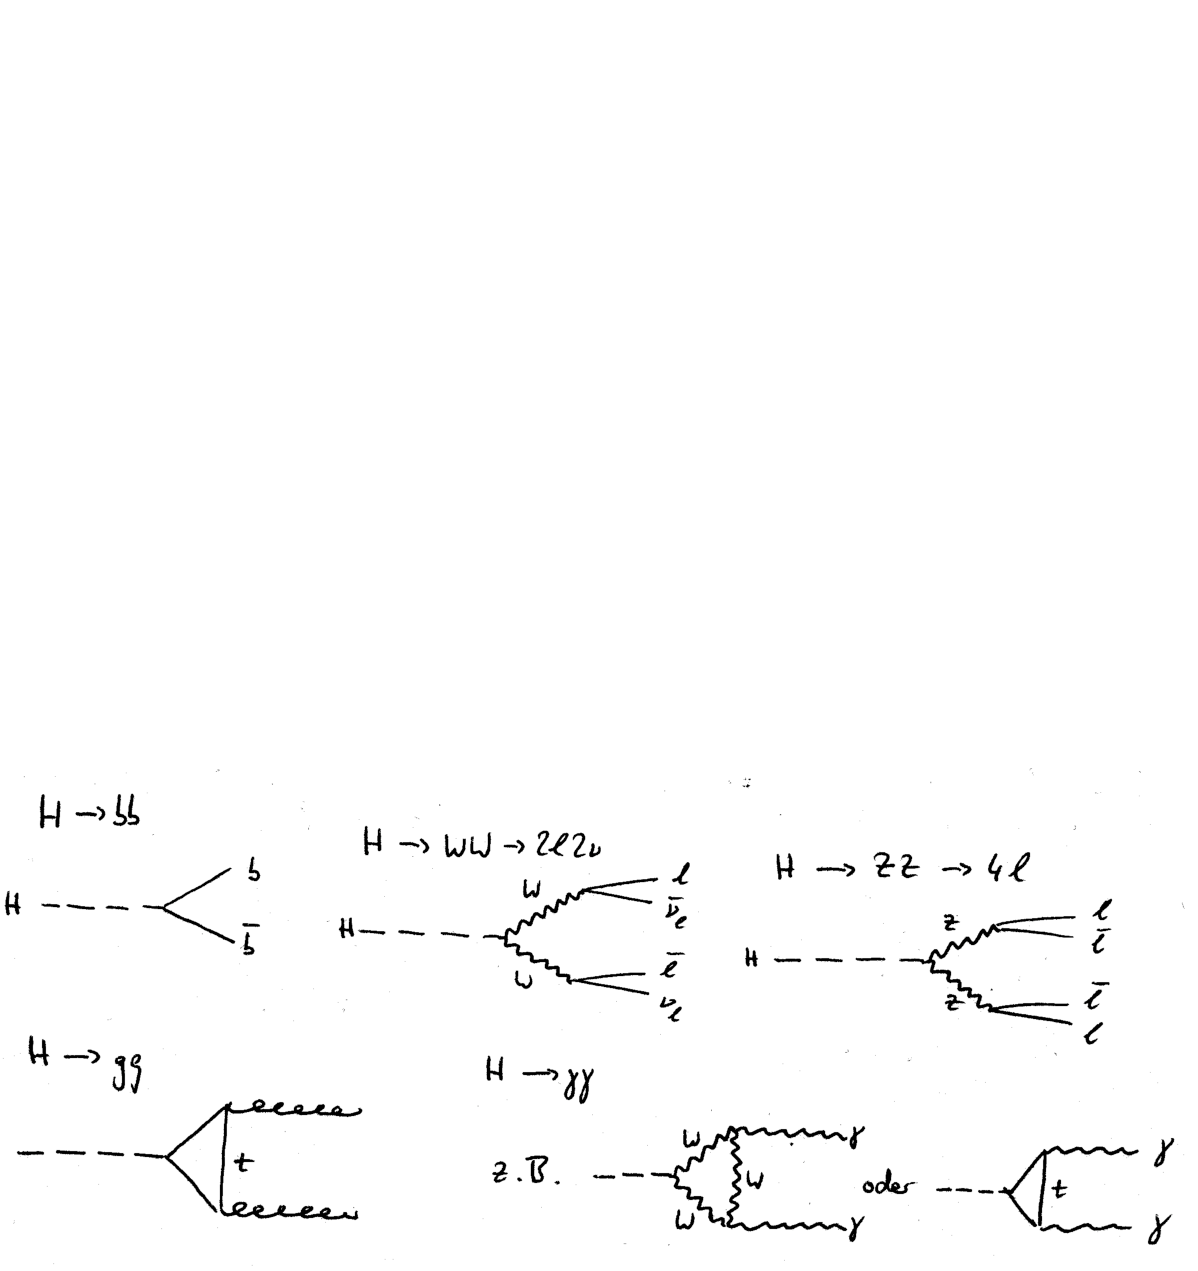
\includegraphics[height=6.5cm]{figures/LsgHiggs_decay.pdf}
		        \end{figure}
The most probable channel is bb because is the only one with one vertex and the interaction vertex of Higgs and fermion is directely proportional to the mass of the fermion therefore the bottom quork is the most probable. All the other particles are too massive for decay just with one vertex and we need loops

}

%\item 
%    Wie viele $pp \to b\bar{b}$ Ereignisse erwarten Sie bei einer integrierten Luminosität
%    von $\SI{50}{fb^{-1}}$? Wie viele Higgs-Ereignisse erwarten Sie in jedem der relevanten Higgs-Zerfallskanäle? 
%    \\(\textit{Hinweis: } Nehmen Sie an, dass der $b\bar{b}$-Wirkungsquerschnitt ungefähr $\SI{1e6}{\nano\barn}$ beträgt und der totale Wirkungsquerschnitt des Higgs bei $\SI{2e-2}{\nano\barn}$ liegt.)
      			
%    \solution{
%    How many $pp \to b\bar{b}$ events do you expect at a integrated luminosity of
	%$\SI{50}{fb^{-1}}$? How many Higgs events do you expect in each Higgs decay channel? (Assume a $b\bar{b}$ cross section of around \SI{1e6}{nb} and total cross section for the Higgs of \SI{2e-2}{nb}.)
   
    %            At an integrated luminosity of $\SI{50}{fb^{-1}}$ and a $bb$-XS
%		        of around \SI{1e6}{nb} you get around \num{5e13} $bb$ events. For a
		        %\SI{125}{GeV} Higgs the total XS is \SI{2e-2}{nb} which is leads to
		        %around \num{1000000} Higgs events.
		        %Around \SI{60}{\percent} (\num{600000} Events) decay through the
		        %$b\overline{b}$ channel, \SI{20}{\percent} through the $WW$ channel,
		        %\SI{7}{\percent} through the $gg$ or $\tau\tau$ channel, \SI{3}{\percent}
		        %through the $c\overline{c}$, or  $ZZ$ channel and \SI{0.2}{\percent}
		        %(\num{2000}) through the $\gamma\gamma$ channel.}
          
\item Die Oberfläche der Erde ist ständig einer großen Menge an energiereichen Teilchen ausgesetzt, die als kosmische Strahlung (CR) bezeichnet wird. Wenn diese CR mit den Molekülen der Atmosphäre in Wechselwirkung tritt, wird eine große Menge subatomarer Teilchen erzeugt, darunter auch das Higgs-Boson. Geht man davon aus, dass die Protonen in den Molekülen der Atmosphäre aufgrund der hohen Energie der CR, die mit diesen Hadronen kollidieren, freie Teilchen sind, können die Kollisionen als Proton-Proton-Kollisionen betrachtet werden. Der dominierende Teil des Wirkungsquerschnitts der Higgs-Produktion ist die Gluonenfusion, und das Verzweigungsverhältnis der Higgs-Bosonen-Produktion durch Gluonenfusion zum gesamten p-p-Wirkungsquerschnitt $\frac{\sigma_{Higgs}}{\sigma_{total}}$ ist in der folgenden Grafik dargestellt

\begin{figure}[htbp]
		            \centering
		            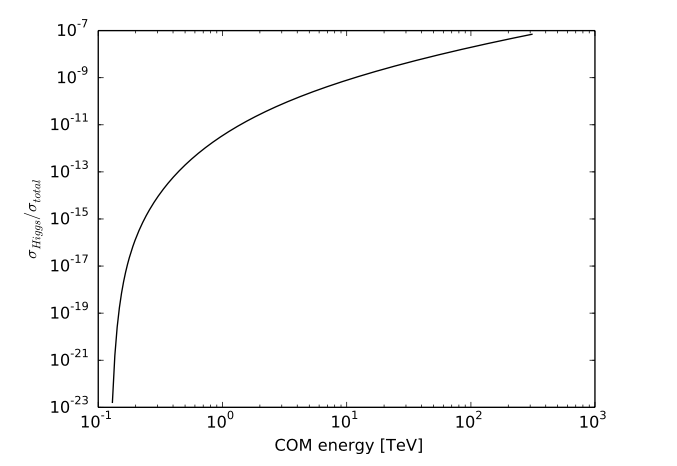
\includegraphics[height=6.5cm]{figures/Higgs_BR}
\end{figure}
Die Anzahl der pro Zeiteinheit $\mathrm{d}t$ erzeugten Higgs-Teilchen $N_H$ ist gleich

\begin{equation}
\frac{\mathrm{d}N_H}{\mathrm{d}t}=\frac{\sigma_{Higgs}}{\sigma_{total}}\frac{\mathrm{d}\phi}{\mathrm{d}t}\,,
\end{equation}
wobei $\frac{\mathrm{d}\phi}{\mathrm{d}t}$ der Fluss von CR pro Zeiteinheit ist und das $\frac{\sigma_{Higgs}}{\sigma_{total}}$ zuvor definiert wurde.
Der Fluss der CR pro Zeiteinheit, Oberfläche $A$, Energie des Massenschwerpunkts der Kollision $E_{COM}$ und Raumwinkel $\mathrm{d}\Omega$ ist gegeben durch
\begin{equation}
\frac{\mathrm{d}\phi^4}{\mathrm{d}t\mathrm{d}A\mathrm{d}E_{COM}\mathrm{d}\Omega}\sim 10^{-9}.
\end{equation}
Schätzen Sie die Anzahl der Higgs-Bosonen ab, die an einem Tag in 10 km Höhe produziert werden, wenn Sie nur CR aus Quellen innerhalb der Galaxie ($E_{CR}\sim \SI{3e10}{\electronvolt}$) berücksichtigen und annehmen, dass der Fluss aus allen Richtungen isotrop ist (keine Abhängigkeit des $\phi$ von der Fläche und dem Raumwinkel).
\textit{(Hinweise: Die Beziehung zwischen der Energie im Massenschwerpunkt und der Energie des CR ist $E_{COM}=\sqrt{(E_{CR} +m_P)2m_P}$. Der Radius der Erde beträgt \SI{6371}{\kilo\meter}. Die Masse des Protoms $m_P$ ist gleich \SI{0.938}{\giga\electronvolt/c^2}.)} (4P)
  \solution{
\begin{equation}
A =(6371 km + 10 km)^2\pi = 1.28 \times 10^{11} m^2
\end{equation}
\begin{equation}
      E_{COM}=\sqrt{(E_{CR} +m_P)2m_P} =2.3\times 10^4 GeV
\end{equation}
      From the graph, the value of $\frac{\sigma_{Higgs}}{\sigma_{total}}$ is approximately $10^{-8}$.
     \begin{align*}
\frac{\mathrm{d}N_H}{\mathrm{d}t}&=\frac{\sigma_{Higgs}}{\sigma_{total}}\times\frac{10^{-9}}{m^2 \times s \times sr \times GeV} \times A \times 4\pi \times E_{COM}\\
&= 10^{-8}\times \frac{10^{-9}}{m^2 \times s \times sr \times GeV} \times 1.28 \times 10^{11} m^2\times 4\pi \times 2.3\times10^4 GeV = 0.36 Higgs\cdot s^{-1}
\end{align*}
In a day there are 86400 seconds, so in one day approximatelly 31k Higgs are produced
  }
\end{enumerate}